% beamer presentation
% Karting report

\documentclass{beamer}
% english language
\usepackage[english]{babel}

% tables
\usepackage{tabularx}
\usepackage{graphicx}
\usepackage{hyperref}
\usepackage{listings}
\usepackage{color}

\usetheme{Madrid}

% unibs color #3d5895
% \definecolor{unibs}{RGB}{61,88,149}
\definecolor{unibs}{HTML}{3d5895}


\setbeamercolor{palette primary}{fg=white, bg=unibs}
\setbeamercolor{palette secondary}{fg=white, bg=unibs}
\setbeamercolor{palette tertiary}{fg=white, bg=unibs}
\setbeamercolor{palette quaternary}{fg=white, bg=unibs}

\title{Karting report}
\author{Denis Festa}
\date{\today}

\begin{document}


\begin{frame}
    \titlepage
    \centering
    
\includegraphics[width=0.2\linewidth]{unibs-circ-logo.pdf}
\end{frame}

\logo{
\includegraphics[width=0.1\linewidth]{unibs_logo.pdf}}


\section*{User groups}

\begin{frame}
\frametitle{User groups}
\begin{figure}
    \centering
    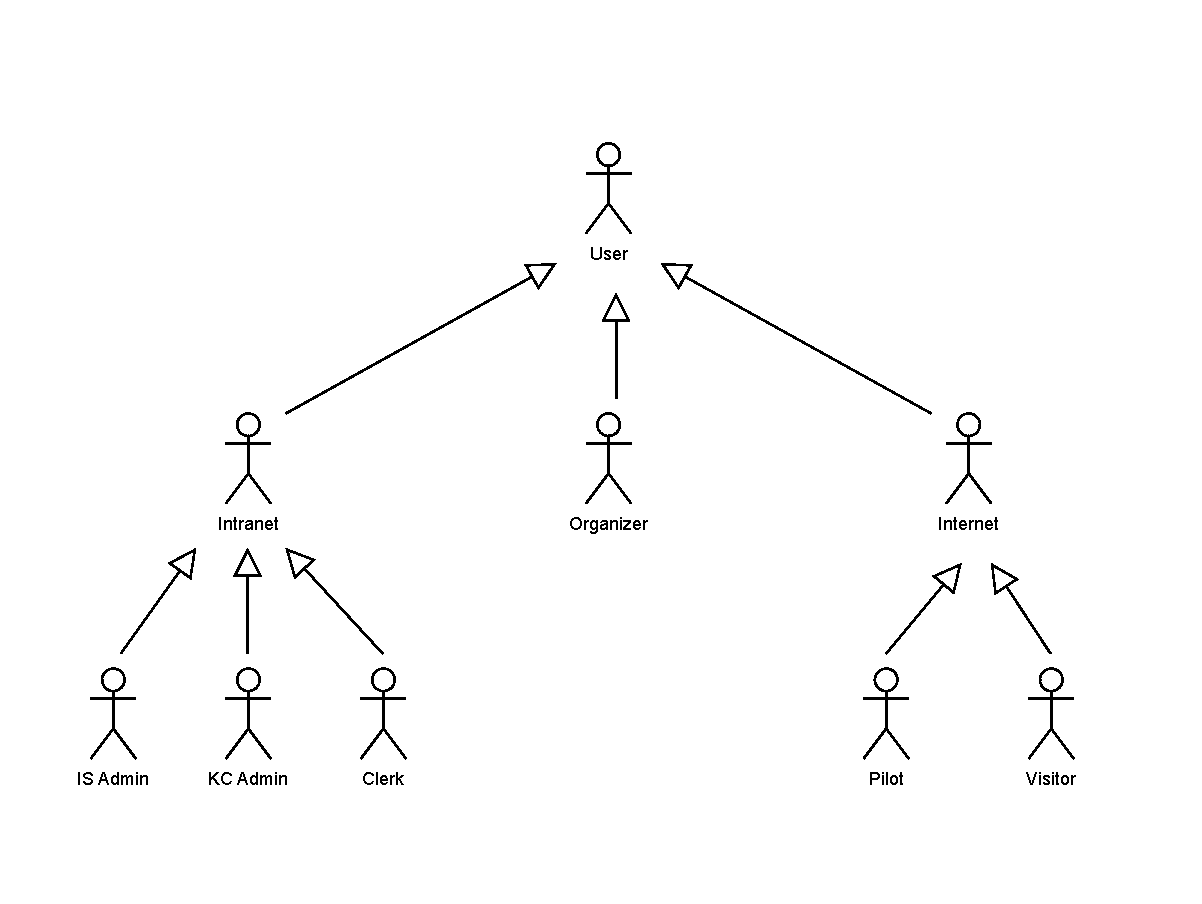
\includegraphics[width=0.8\linewidth]{drawio/users-uc.pdf}
    % \caption{User groups}
\end{figure}
\end{frame}

\section*{Use cases}

\subsection*{User}

\begin{frame}
    \frametitle{User}
    \centering
    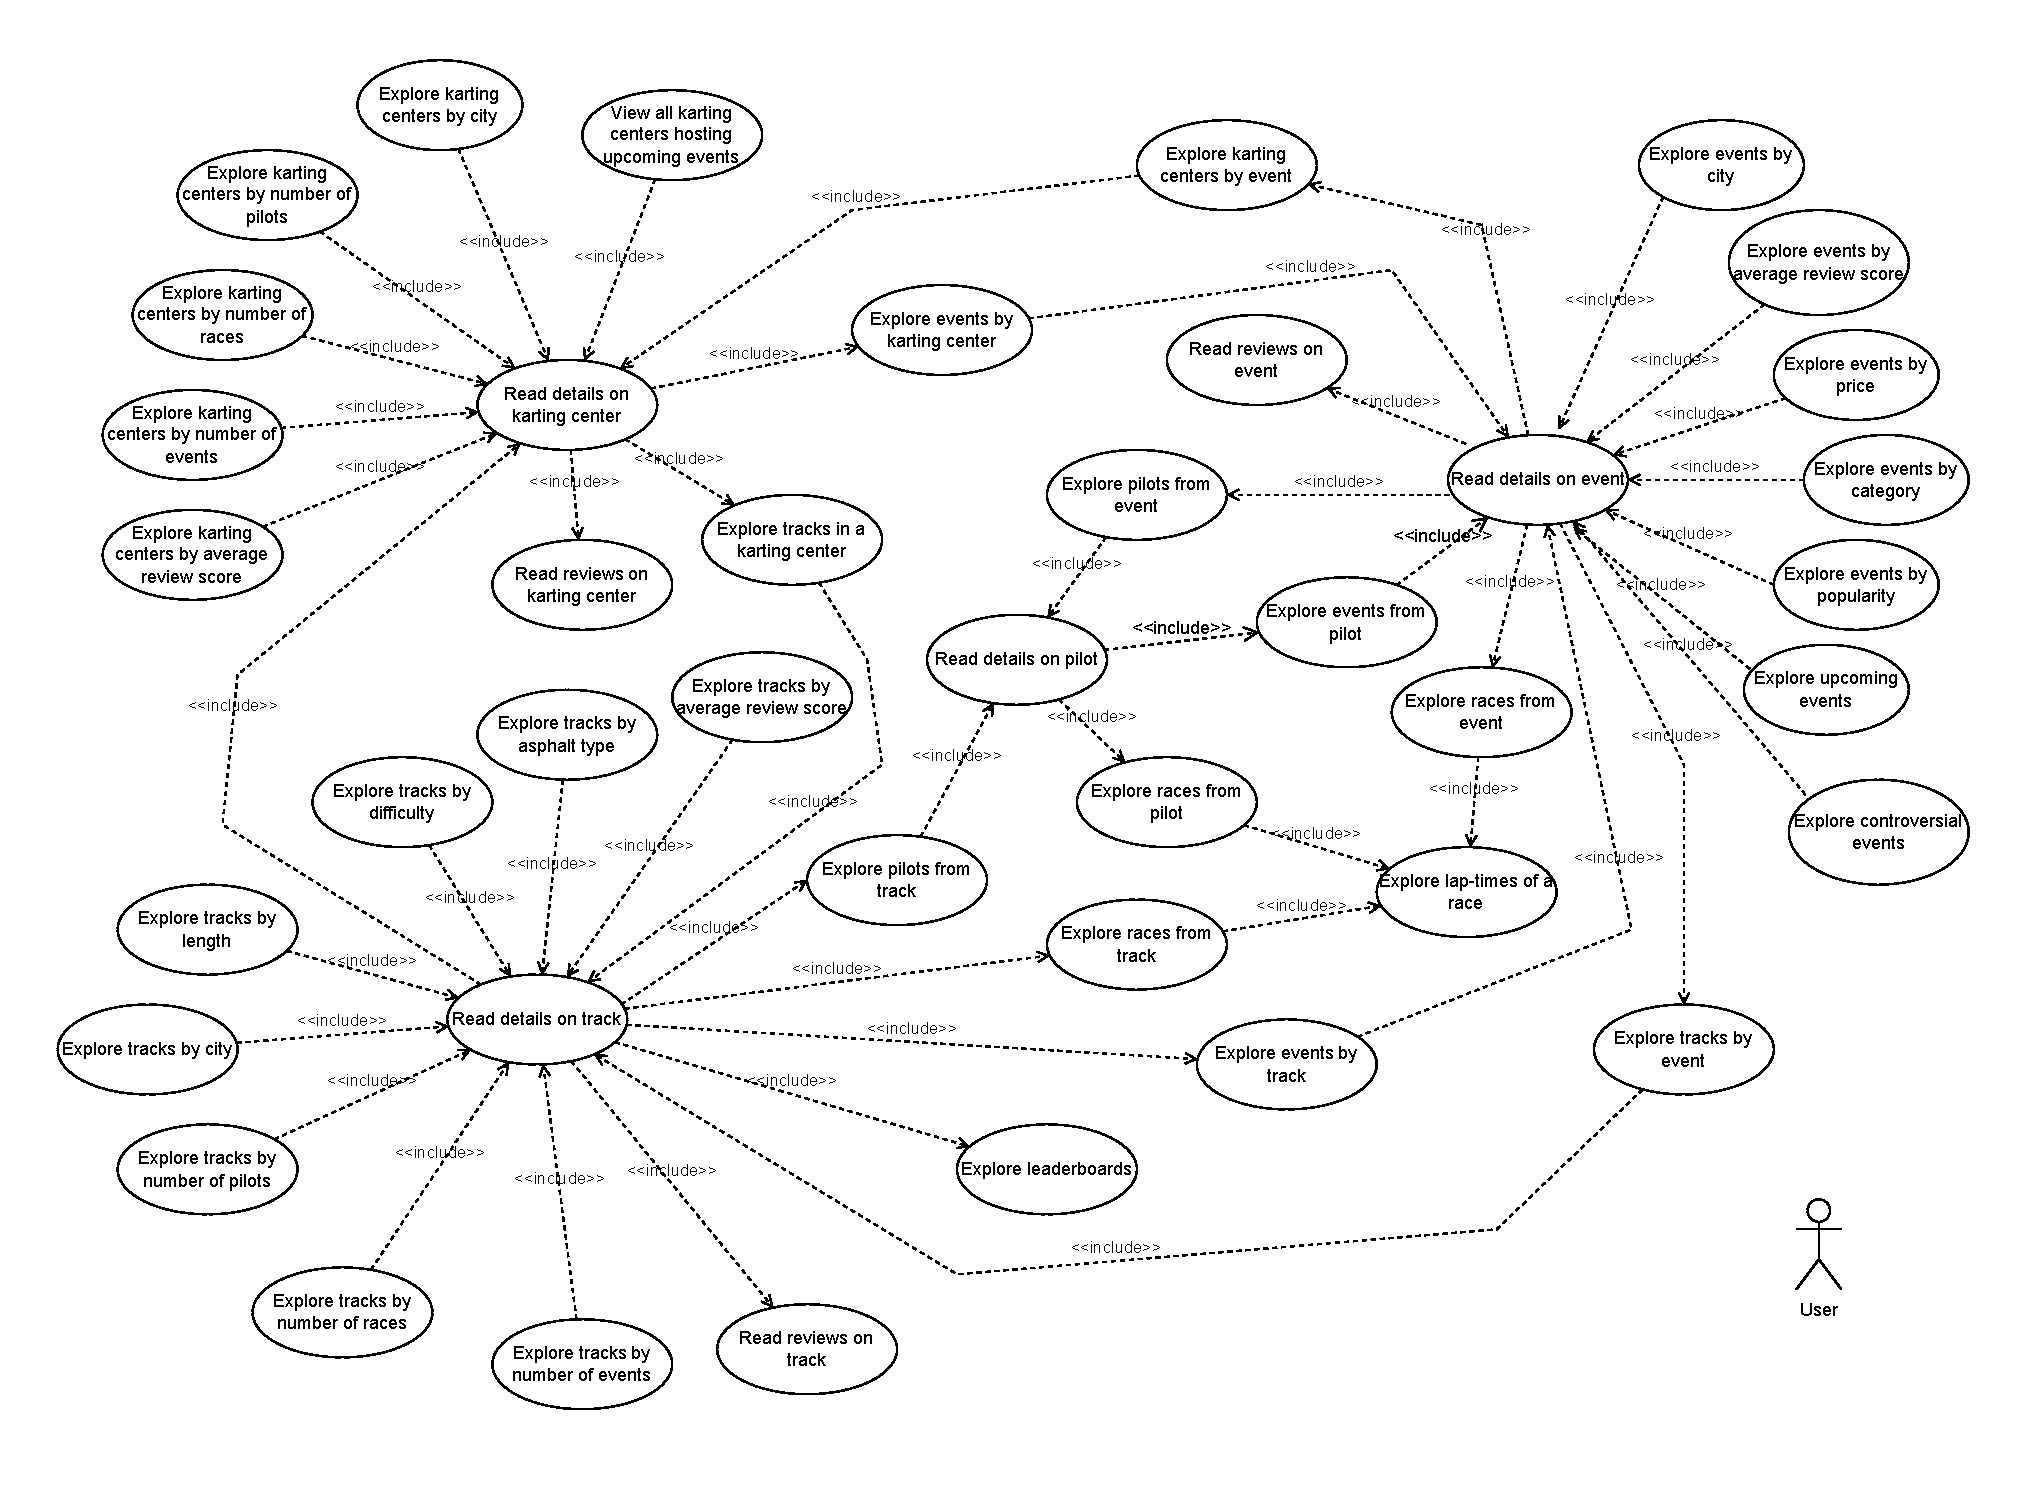
\includegraphics[width=0.8\linewidth]{drawio/user.pdf}
\end{frame}

% %%%%%%%%%% KARTING CENTER AREA %%%%%%%%%%%%%%%

\begin{frame}
\frametitle{Specification sheet}
\begin{table}
    \tiny
    \begin{tabular}{|p{2cm}|p{6cm}|}
    \hline
    Title & \textbf{Explore karting centers by city} \\
    \hline
    Goal & The user seeks karting centers selecting one city at a time. \\
    \hline
    Precondition & The user is in the area (of the public view) dedicated to karting centers.\\
    \hline
    Postcondition & The user obtains the list of karting centers from which he can move on.\\
    \hline
    Workflow &
    - The user moves to the area dedicated to karting centers. \newline
    - The user selects a city. \\
    \hline
    \end{tabular}
\end{table}
\end{frame}

\begin{frame}
    \frametitle{Specification sheet}
    \begin{table}
        \tiny
        \begin{tabular}{|p{2cm}|p{6cm}|}
        \hline
        Title & \textbf{Explore karting centers by number of races} \\
        \hline
        Goal & The user seeks karting centers selecting one range of number of races (that
        were hosted on any of the tracks of the karting center) at a time. \\
        \hline
        Precondition & The user is in the area (of the public view) dedicated to karting centers.\\
        \hline
        Postcondition & The user obtains the list of karting centers from which he can move on.\\
        \hline
        Workflow &
        - The user moves to the area dedicated to karting centers. \newline
        - The user selects a range of number of races. \\
        \hline
        \end{tabular}
\end{table}
\end{frame}


\begin{frame}
    \frametitle{Specification sheet}
    \begin{table}
        \tiny
        \begin{tabular}{|p{2cm}|p{6cm}|}
        \hline
        Title & \textbf{Explore karting centers by number of pilots} \\
        \hline
        Goal & The user seeks karting centers selecting one range of number of pilots (who had a race on 
        any of the tracks of the karting center) at a time. \\
        \hline
        Precondition & The user is in the area (of the public view) dedicated to karting centers.\\
        \hline
        Postcondition & The user obtains the list of karting centers from which he can move on.\\
        \hline
        Workflow &
        - The user moves to the area dedicated to karting centers. \newline
        - The user selects a range of number of pilots. \\
        \hline
        \end{tabular}
\end{table}
\end{frame}

\begin{frame}
    \frametitle{Specification sheet}
    \begin{table}
        \tiny
        \begin{tabular}{|p{2cm}|p{6cm}|}
        \hline
        Title & \textbf{Explore karting centers by number of events} \\
        \hline
        Goal & The user seeks karting centers selecting one range of number of events (that had
        at least one race hosted on 
        any of the tracks of the karting center) at a time. \\
        \hline
        Precondition & The user is in the area (of the public view) dedicated to karting centers.\\
        \hline
        Postcondition & The user obtains the list of karting centers from which he can move on.\\
        \hline
        Workflow &
        - The user moves to the area dedicated to karting centers. \newline
        - The user selects a range of number of events. \\
        \hline
        \end{tabular}
\end{table}
\end{frame}

\begin{frame}
    \frametitle{Specification sheet}
    \begin{table}
        \tiny
        \begin{tabular}{|p{2cm}|p{6cm}|}
        \hline
        Title & \textbf{Explore karting centers by average review score} \\
        \hline
        Goal & The user seeks karting centers selecting one range of average review scores (given to the karting center by all the pilots
        that had at least one race on one of the tracks of the karting center) at a time. \\
        \hline
        Precondition & The user is in the area (of the public view) dedicated to karting centers.\\
        \hline
        Postcondition & The user obtains the list of karting centers from which he can move on.\\
        \hline
        Workflow &
        - The user moves to the area dedicated to karting centers. \newline
        - The user selects a range of scores (the ranges are the same for karting centes, tracks and events). \\
        \hline
        \end{tabular}
\end{table}
\end{frame}

\begin{frame}
    \frametitle{Specification sheet}
    \begin{table}
        \tiny
        \begin{tabular}{|p{2cm}|p{6cm}|}
        \hline
        Title & \textbf{View all karting centers hosting upcoming events} \\
        \hline
        Goal & The user scrolls through the list of karting centers that are going to host an upcoming event. \\
        \hline
        Precondition & The user already has this information in the homepage.\\
        \hline
        Postcondition & The user obtains the list of karting centers from which he can move on.\\
        \hline
        Workflow &
        - The user reaches the homepage. \\
        \hline
        \end{tabular}
\end{table}
\end{frame}

\begin{frame}
    \frametitle{Specification sheet}
    \begin{table}
        \tiny
        \begin{tabular}{|p{2cm}|p{6cm}|}
        \hline
        Title & \textbf{Read details on karting center} \\
        \hline
        Goal & The user chooses one karting center to focus on and reads its details. \\
        \hline
        Precondition & The user chose a karting center from a list of karting centers (obtained from any of the previous use cases).\\
        \hline
        Postcondition & The user obtains the details on the karting center and can move on to other related informations (e.g. tracks, reviews)\\
        \hline
        Workflow &
        - The user chooses one karting center from a list. \\
        \hline
        \end{tabular}
\end{table}
\end{frame}

\begin{frame}
    \frametitle{Specification sheet}
    \begin{table}
        \tiny
        \begin{tabular}{|p{2cm}|p{6cm}|}
        \hline
        Title & \textbf{Read reviews on karting center} \\
        \hline
        Goal & The user chooses one karting center to focus on and scrolls the reviews it received (from pilots
        that had at least one race on one track of the karting center). \\
        \hline
        Precondition & The user chose a karting center from a list of karting centers (obtained from any of the previous use cases).\\
        \hline
        Postcondition & The user obtains the reviews on the karting center in the area dedicated to reviews. \\
        \hline
        Workflow &
        - The user moves from the page dedicated to the details of the karting center to the
        page dedicated to reviews through a click. \\
        \hline
        \end{tabular}
\end{table}
\end{frame}

\begin{frame}
    \frametitle{Specification sheet}
    \begin{table}
        \tiny
        \begin{tabular}{|p{2cm}|p{6cm}|}
        \hline
        Title & \textbf{Explore tracks in a karting center} \\
        \hline
        Goal & The user chooses one karting center to focus on and explores the tracks it offers. \\
        \hline
        Precondition & The user chose a karting center from a list of karting centers (obtained from any of the previous use cases).\\
        \hline
        Postcondition & The user obtains the tracks offered by the karting center in the area dedicated to tracks. \\
        \hline
        Workflow &
        - The user moves from the page dedicated to the details of the karting center to the
        page dedicated to tracks through a click. \\
        \hline
        \end{tabular}
\end{table}
\end{frame}

\begin{frame}
    \frametitle{Specification sheet}
    \begin{table}
        \tiny
        \begin{tabular}{|p{2cm}|p{6cm}|}
        \hline
        Title & \textbf{Explore tracks by asphalt type} \\
        \hline
        Goal & The user seeks tracks selecting one asphalt type at a time. \\
        \hline
        Precondition & The user is in the area (of the public view) dedicated to tracks.\\
        \hline
        Postcondition & The user obtains the list of tracks from which he can move on.\\
        \hline
        Workflow &
        - The user moves to the area dedicated to tracks. \newline
        - The user selects an asphalt type. \\
        \hline
        \end{tabular}
\end{table}
\end{frame}

\begin{frame}
    \frametitle{Specification sheet}
    \begin{table}
        \tiny
        \begin{tabular}{|p{2cm}|p{6cm}|}
        \hline
        Title & \textbf{Explore tracks by difficulty} \\
        \hline
        Goal & The user seeks tracks selecting one difficulty at a time. \\
        \hline
        Precondition & The user is in the area (of the public view) dedicated to tracks.\\
        \hline
        Postcondition & The user obtains the list of tracks from which he can move on.\\
        \hline
        Workflow &
        - The user moves to the area dedicated to tracks. \newline
        - The user selects a difficulty. \\
        \hline
        \end{tabular}
\end{table}
\end{frame}

\begin{frame}
    \frametitle{Specification sheet}
    \begin{table}
        \tiny
        \begin{tabular}{|p{2cm}|p{6cm}|}
        \hline
        Title & \textbf{Explore tracks by length} \\
        \hline
        Goal & The user seeks tracks selecting one range of lengths at a time. \\
        \hline
        Precondition & The user is in the area (of the public view) dedicated to tracks.\\
        \hline
        Postcondition & The user obtains the list of tracks from which he can move on.\\
        \hline
        Workflow &
        - The user moves to the area dedicated to tracks. \newline
        - The user selects a range of lengths. \\
        \hline
        \end{tabular}
\end{table}
\end{frame}

\begin{frame}
    \frametitle{Specification sheet}
    \begin{table}
        \tiny
        \begin{tabular}{|p{2cm}|p{6cm}|}
        \hline
        Title & \textbf{Explore tracks by city} \\
        \hline
        Goal & The user seeks tracks selecting one city at a time. \\
        \hline
        Precondition & The user is in the area (of the public view) dedicated to tracks.\\
        \hline
        Postcondition & The user obtains the list of tracks from which he can move on.\\
        \hline
        Workflow &
        - The user moves to the area dedicated to tracks. \newline
        - The user selects a city. \\
        \hline
        \end{tabular}
\end{table}
\end{frame}

\begin{frame}
    \frametitle{Specification sheet}
    \begin{table}
        \tiny
        \begin{tabular}{|p{2cm}|p{6cm}|}
        \hline
        Title & \textbf{Explore tracks by number of races} \\
        \hline
        Goal & The user seeks tracks selecting one range of number of races
        (that took place on the track) at a time. \\ 
        \hline
        Precondition & The user is in the area (of the public view) dedicated to tracks.\\
        \hline
        Postcondition & The user obtains the list of tracks from which he can move on.\\
        \hline
        Workflow &
        - The user moves to the area dedicated to tracks. \newline
        - The user selects a range of number of races. \\
        \hline
        \end{tabular}
\end{table}
\end{frame}

\begin{frame}
    \frametitle{Specification sheet}
    \begin{table}
        \tiny
        \begin{tabular}{|p{2cm}|p{6cm}|}
        \hline
        Title & \textbf{Explore tracks by number of pilots} \\
        \hline
        Goal & The user seeks tracks selecting one range of number of pilots
        (who had a race on the track) at a time. \\
        \hline
        Precondition & The user is in the area (of the public view) dedicated to tracks.\\
        \hline
        Postcondition & The user obtains the list of tracks from which he can move on.\\
        \hline
        Workflow &
        - The user moves to the area dedicated to tracks. \newline
        - The user selects a range of number of pilots. \\
        \hline
        \end{tabular}
\end{table}
\end{frame}


\begin{frame}
    \frametitle{Specification sheet}
    \begin{table}
        \tiny
        \begin{tabular}{|p{2cm}|p{6cm}|}
        \hline
        Title & \textbf{Explore tracks by number of events} \\
        \hline
        Goal & The user seeks tracks selecting one range of number of events
        (that had at least one race hosted on the track) at a time. \\
        \hline
        Precondition & The user is in the area (of the public view) dedicated to tracks.\\
        \hline
        Postcondition & The user obtains the list of tracks from which he can move on.\\
        \hline
        Workflow &
        - The user moves to the area dedicated to tracks. \newline
        - The user selects a range of number of events. \\
        \hline
        \end{tabular}
\end{table}
\end{frame}

\begin{frame}
    \frametitle{Specification sheet}
    \begin{table}
        \tiny
        \begin{tabular}{|p{2cm}|p{6cm}|}
        \hline
        Title & \textbf{Explore tracks by average review score} \\
        \hline
        Goal & The user seeks tracks selecting one range of average review scores (given to the track by all the pilots
        that had at least one race on the track) at a time. \\
        \hline
        Precondition & The user is in the area (of the public view) dedicated to tracks.\\
        \hline
        Postcondition & The user obtains the list of tracks from which he can move on.\\
        \hline
        Workflow &
        - The user moves to the area dedicated to tracks. \newline
        - The user selects a range of scores (the ranges are the same for karting centes, tracks and events). \\
        \hline
        \end{tabular}
\end{table}
\end{frame}

\begin{frame}
    \frametitle{Specification sheet}
    \begin{table}
        \tiny
        \begin{tabular}{|p{2cm}|p{6cm}|}
        \hline
        Title & \textbf{Read details on track} \\
        \hline
        Goal & The user chooses one track to focus on and reads its details. \\
        \hline
        Precondition & The user chose a track from a list of tracks (obtained from any of the previous use cases).\\
        \hline
        Postcondition & The user obtains the details on the track and can move on to other related informations (e.g. pilots, leaderboards, races, reviews)\\
        \hline
        Workflow &
        - The user chooses one karting center from a list. \\
        \hline
        \end{tabular}
\end{table}
\end{frame}

\begin{frame}
    \frametitle{Specification sheet}
    \begin{table}
        \tiny
        \begin{tabular}{|p{2cm}|p{6cm}|}
        \hline
        Title & \textbf{Read reviews on track} \\
        \hline
        Goal & The user chooses one track to focus on and scrolls the reviews it received (from pilots
        that had at least one race on it). \\
        \hline
        Precondition & The user chose a track from a list of tracks (obtained from any of the previous use cases).\\
        \hline
        Postcondition & The user obtains the reviews on the tracks in the area dedicated to reviews. \\
        \hline
        Workflow &
        - The user moves from the area dedicated to the details of the track to the
        area dedicated to reviews through a click. \\
        \hline
        \end{tabular}
\end{table}
\end{frame}

\begin{frame}
    \frametitle{Specification sheet}
    \begin{table}
        \tiny
        \begin{tabular}{|p{2cm}|p{6cm}|}
        \hline
        Title & \textbf{Explore leaderboards} \\
        \hline
        Goal & The user chooses one track to focus on and explores the leaderboards associated
        to the track (leaderboards are filtering on the whole record of laptimes obtained by pilots in a race,
        a leaderboard can focus on the last month, the last year, sex, weight...) \\
        \hline
        Precondition & The user chose a track from a list of tracks (obtained from any of the previous use cases).\\
        \hline
        Postcondition & The user obtains the list of leaderboards in the area dedicated to leaderboards. \\
        \hline
        Workflow &
        - The user moves from the area dedicated to the details of the track to the
        area dedicated to leaderboards through a click. \\
        \hline
        \end{tabular}
\end{table}
\end{frame}

\begin{frame}
    \frametitle{Specification sheet}
    \begin{table}
        \tiny
        \begin{tabular}{|p{2cm}|p{6cm}|}
        \hline
        Title & \textbf{Explore races from track} \\
        \hline
        Goal & The user chooses one track to focus on and explores the races that took place on the track. \\
        \hline
        Precondition & The user chose a track from a list of tracks (obtained from any of the previous use cases).\\
        \hline
        Postcondition & The user obtains the list of races in the area dedicated to races. \\
        \hline
        Workflow &
        - The user moves from the area dedicated to the details of the track to the
        area dedicated to races through a click. \\
        \hline
        \end{tabular}
\end{table}
\end{frame}

\begin{frame}
    \frametitle{Specification sheet}
    \begin{table}
        \tiny
        \begin{tabular}{|p{2cm}|p{6cm}|}
        \hline
        Title & \textbf{Explore lap-times of a race} \\
        \hline
        Goal & The user chooses one race to focus on and reads all the lap-times made by all the pilots 
        that participated to the race.\\
        \hline
        Precondition & The user chose a race from a list of races (obtained from a track, an event or a pilot).\\
        \hline
        Postcondition & The user obtains the list of lap-times in the area dedicated to lap-times. \\
        \hline
        Workflow &
        - The user moves from the area dedicated to the details of the race to the
        area dedicated to lap-times through a click. \\
        \hline
        \end{tabular}
\end{table}
\end{frame}

\begin{frame}
    \frametitle{Specification sheet}
    \begin{table}
        \tiny
        \begin{tabular}{|p{2cm}|p{6cm}|}
        \hline
        Title & \textbf{Explore pilots from track} \\
        \hline
        Goal & The user chooses one track to focus on and explores the pilots that had at least one race on the track. \\
        \hline
        Precondition & The user chose a track from a list of tracks (obtained from any of the previous use cases).\\
        \hline
        Postcondition & The user obtains the list of pilots in the area dedicated to pilots. \\
        \hline
        Workflow &
        - The user moves from the area dedicated to the details of the track to the
        area dedicated to pilots through a click. \\
        \hline
        \end{tabular}
\end{table}
\end{frame}

\begin{frame}
    \frametitle{Specification sheet}
    \begin{table}
        \tiny
        \begin{tabular}{|p{2cm}|p{6cm}|}
        \hline
        Title & \textbf{Read details on pilot} \\
        \hline
        Goal & The user chooses one pilot to focus on and reads its details. \\
        \hline
        Precondition & The user chose a pilot from a list of pilots (obtained from a track, a race, an event).\\
        \hline
        Postcondition & The user obtains the details on the pilot and can move on to other related informations (e.g. races, events). \\
        \hline
        Workflow &
        - The user chooses one pilot from a list. \\
        \hline
        \end{tabular}
\end{table}
\end{frame}

\begin{frame}
    \frametitle{Specification sheet}
    \begin{table}
        \tiny
        \begin{tabular}{|p{2cm}|p{6cm}|}
        \hline
        Title & \textbf{Explore events from pilot} \\
        \hline
        Goal & The user chooses one pilot to focus on and explores the events that the pilot attended. \\
        \hline
        Precondition & The user chose a pilot from a list of pilots (obtained from a track, a race, an event).\\
        \hline
        Postcondition & The user obtains a list of events in the area dedicated to events. \\
        \hline
        Workflow &
        - The user moves from the area dedicated to the details of the pilot to the
        area dedicated to events through a click. \\
        \hline
        \end{tabular}
\end{table}
\end{frame}

\begin{frame}
    \frametitle{Specification sheet}
    \begin{table}
        \tiny
        \begin{tabular}{|p{2cm}|p{6cm}|}
        \hline
        Title & \textbf{Explore races from pilot} \\
        \hline
        Goal & The user chooses one pilot to focus on and explores the races that the pilot had. \\
        \hline
        Precondition & The user chose a pilot from a list of pilots (obtained from a track, a race, an event).\\
        \hline
        Postcondition & The user obtains a list of races in the area dedicated to races. \\
        \hline
        Workflow &
        - The user moves from the area dedicated to the details of the pilot to the
        area dedicated to races through a click. \\
        \hline
        \end{tabular}
\end{table}
\end{frame}

% EXPLORE EVENTS

\begin{frame}
    \frametitle{Specification sheet}
    \begin{table}
        \tiny
        \begin{tabular}{|p{2cm}|p{6cm}|}
        \hline
        Title & \textbf{Explore events by city} \\
        \hline
        Goal & The user explres events selecting one city at a time. \\
        \hline
        Precondition & The user is in the area (of the public view) dedicated to events.\\
        \hline
        Postcondition & The user obtains the list of events from which he can move on.\\
        \hline
        Workflow &
        - The user moves to the area dedicated to events. \newline
        - The user selects a city. \\
        \hline
        \end{tabular}
\end{table}
\end{frame}


\begin{frame}
    \frametitle{Specification sheet}
    \begin{table}
        \tiny
        \begin{tabular}{|p{2cm}|p{6cm}|}
        \hline
        Title & \textbf{Explore events by average review score} \\
        \hline
        Goal & The user explores events selecting one range of average review scores (given to the event by all the pilots
        that partecipated to it) at a time. \\
        \hline
        Precondition & The user is in the area (of the public view) dedicated to events.\\
        \hline
        Postcondition & The user obtains the list of events from which he can move on.\\
        \hline
        Workflow &
        - The user moves to the area dedicated to events. \newline
        - The user selects a range of scores (the ranges are the same for karting centes, tracks and events). \\
        \hline
        \end{tabular}
\end{table}
\end{frame}

\begin{frame}
    \frametitle{Specification sheet}
    \begin{table}
        \tiny
        \begin{tabular}{|p{2cm}|p{6cm}|}
        \hline
        Title & \textbf{Explore events by price} \\
        \hline
        Goal & The user explores events selecting one range of prices at a time. \\
        \hline
        Precondition & The user is in the area (of the public view) dedicated to events.\\
        \hline
        Postcondition & The user obtains the list of events from which he can move on.\\
        \hline
        Workflow &
        - The user moves to the area dedicated to events. \newline
        - The user selects a range of prices. \\
        \hline
        \end{tabular}
\end{table}
\end{frame}

\begin{frame}
    \frametitle{Specification sheet}
    \begin{table}
        \tiny
        \begin{tabular}{|p{2cm}|p{6cm}|}
        \hline
        Title & \textbf{Explore events by category} \\
        \hline
        Goal & The user explores events selecting one category at a time. \\
        \hline
        Precondition & The user is in the area (of the public view) dedicated to events.\\
        \hline
        Postcondition & The user obtains the list of events from which he can move on.\\
        \hline
        Workflow &
        - The user moves to the area dedicated to events. \newline
        - The user selects a category. \\
        \hline
        \end{tabular}
\end{table}
\end{frame}

\begin{frame}
    \frametitle{Specification sheet}
    \begin{table}
        \tiny
        \begin{tabular}{|p{2cm}|p{6cm}|}
        \hline
        Title & \textbf{Explore events by popularity} \\
        \hline
        Goal & The user explores only the events considered popular (those that have
        at least $N$ partecipants and $M$ reviews) \\
        \hline
        Precondition & The user is in the area (of the public view) dedicated to events.\\
        \hline
        Postcondition & The user obtains the list of events from which he can move on.\\
        \hline
        Workflow &
        - The user moves to the area dedicated to events. \newline
        - The user chooses an event from the list of popular events already provided in the area
        dedicated to events. \\
        \hline
        \end{tabular}
\end{table}
\end{frame}

\begin{frame}
    \frametitle{Specification sheet}
    \begin{table}
        \tiny
        \begin{tabular}{|p{2cm}|p{6cm}|}
        \hline
        Title & \textbf{Explore upcoming events} \\
        \hline
        Goal & The user explores only the upcoming events (those whose first race still has to take place). \\
        \hline
        Precondition & The user is in the area (of the public view) dedicated to events or in the homepage (which 
        already shows the list of upcoming events, the list of tracks that will be involved and the list of 
        karting centers that will be involved). \\
        \hline
        Postcondition & The user obtains the list of events from which he can move on.\\
        \hline
        Workflow &
        - A: the user chooses an event from the list of upcoming events already provided in the homepage.\newline
        - B.1: the user moves to the area dedicated to events. \newline
        - B.2: the user chooses an event from the list of upcoming events already provided in the area dedicated
        to events. \\
        \hline
        \end{tabular}
\end{table}
\end{frame}

\begin{frame}
    \frametitle{Specification sheet}
    \begin{table}
        \tiny
        \begin{tabular}{|p{2cm}|p{6cm}|}
        \hline
        Title & \textbf{Explore controversial events} \\
        \hline
        Goal & The user explores only the controversial events (those that have at least $N$ reviews under 25\% of the maximum score
        and at least $M$ reviews over 75\% of the maximum score). \\
        \hline
        Precondition & The user is in the area (of the public view) dedicated to events.\\
        \hline
        Postcondition & The user obtains the list of events from which he can move on.\\
        \hline
        Workflow &
        - The user moves to the area dedicated to events. \newline
        - The user chooses an event from the list of controversial events already provided in the area dedicated to events. \\
        \hline
        \end{tabular}
\end{table}
\end{frame}

\begin{frame}
    \frametitle{Specification sheet}
    \begin{table}
        \tiny
        \begin{tabular}{|p{2cm}|p{6cm}|}
        \hline
        Title & \textbf{Read details on event} \\
        \hline
        Goal & The user chooses one event to focus on and reads its details. \\
        \hline
        Precondition & The user chose an event from a list of events (obtained from any of the previous use cases).\\
        \hline
        Postcondition & The user obtains the details on the event and can move on to other related
        informations (e.g. races, pilots) \\
        \hline
        Workflow &
        - The user chooses one event from a list. \\
        \hline
        \end{tabular}
\end{table}
\end{frame}

\begin{frame}
    \frametitle{Specification sheet}
    \begin{table}
        \tiny
        \begin{tabular}{|p{2cm}|p{6cm}|}
        \hline  
        Title & \textbf{Explore pilots from event} \\
        \hline
        Goal & The user chooses one event to focus on and explores the pilots that partecipated to the event. \\
        \hline
        Precondition & The user chose an event from a list of events (obtained from any of the previous use cases).\\
        \hline
        Postcondition & The user obtains a list of pilots in the area dedicated to pilots. \\
        \hline
        Workflow &
        - The user moves from the area dedicated to the details of the event to the
        area dedicated to pilots through a click. \\
        \hline
        \end{tabular}
\end{table}
\end{frame}

\begin{frame}
    \frametitle{Specification sheet}
    \begin{table}
        \tiny
        \begin{tabular}{|p{2cm}|p{6cm}|}
        \hline  
        Title & \textbf{Read reviews on event} \\
        \hline
        Goal & The user chooses one event to focus on and scrolls the reviews it received (from pilots that 
        participated to the event). \\
        \hline
        Precondition & The user chose an event from a list of events (obtained from any of the previous use cases).\\
        \hline
        Postcondition & The user obtains the reviews on the event in the area dedicated to reviews. \\
        \hline
        Workflow &
        - The user moves from the area dedicated to the details of the event to the
        area dedicated to reviews through a click. \\
        \hline
        \end{tabular}
\end{table}
\end{frame}



% %%%%% EVENT DETAILS, RACES FROM EVENT, PILOTS FROM EVENT, REVIEWS ON EVENT


% 
% 
% 
% 
% INTRANET
% 
% 
% 
% 

\subsection*{Intranet}

\begin{frame}
    \frametitle{Intranet}
    \centering
    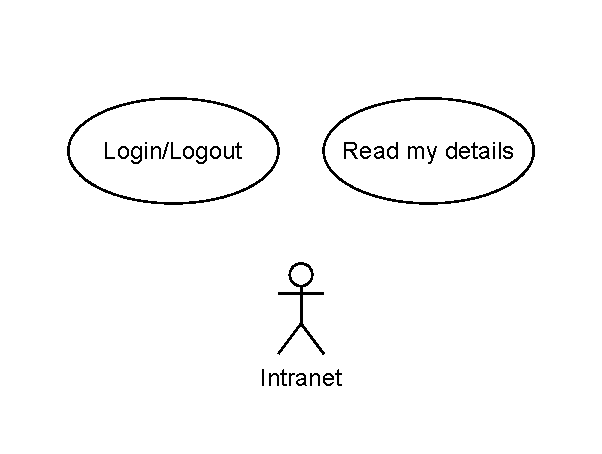
\includegraphics[width=0.7\linewidth]{drawio/intranet.pdf}
\end{frame}

\begin{frame}
    \frametitle{Karting center administrator}
    \centering
    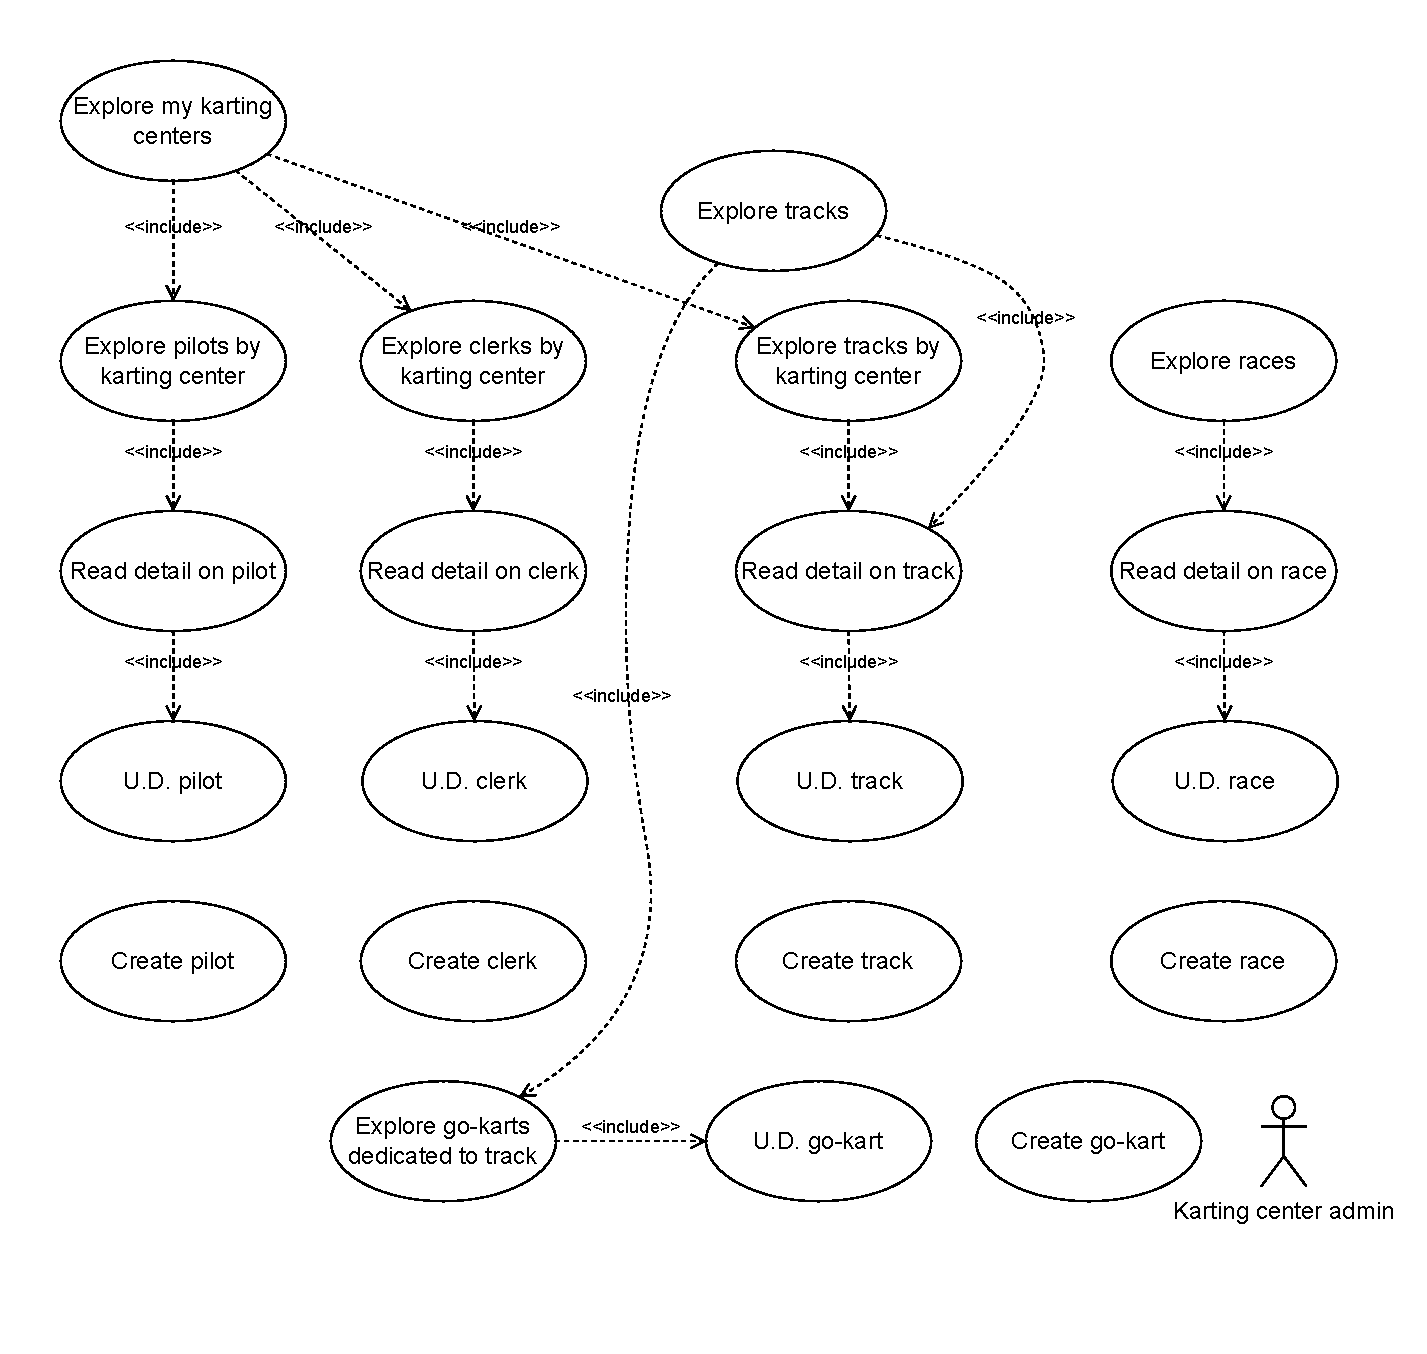
\includegraphics[width=0.7\linewidth]{drawio/karting-center-admin.pdf}
\end{frame}

\begin{frame}
    \frametitle{Clerk}
    \centering
    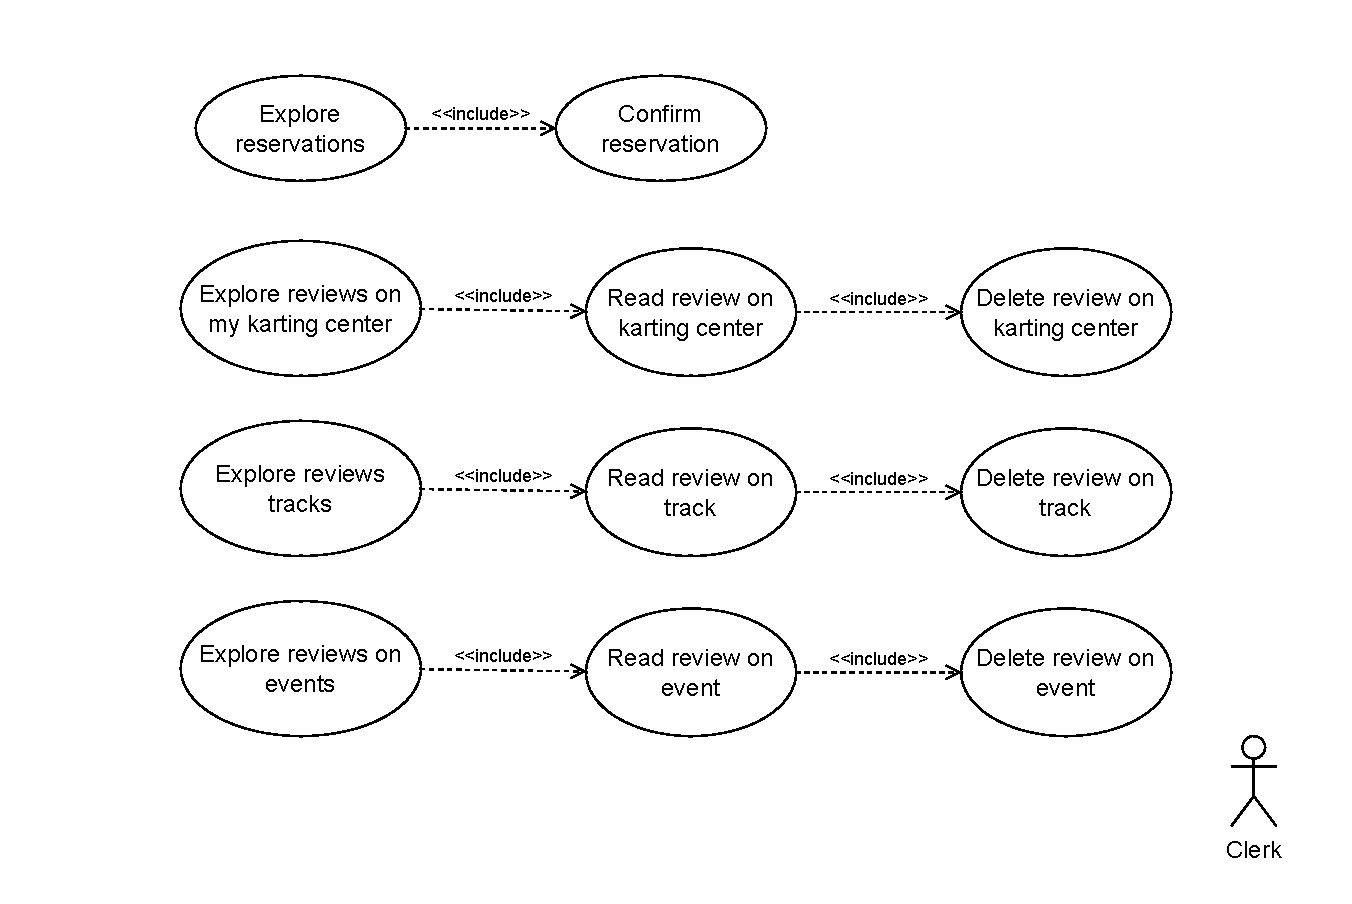
\includegraphics[width=0.9\linewidth]{drawio/clerk.pdf}
\end{frame}

\begin{frame}
    \frametitle{Information system administrator}
    \centering
    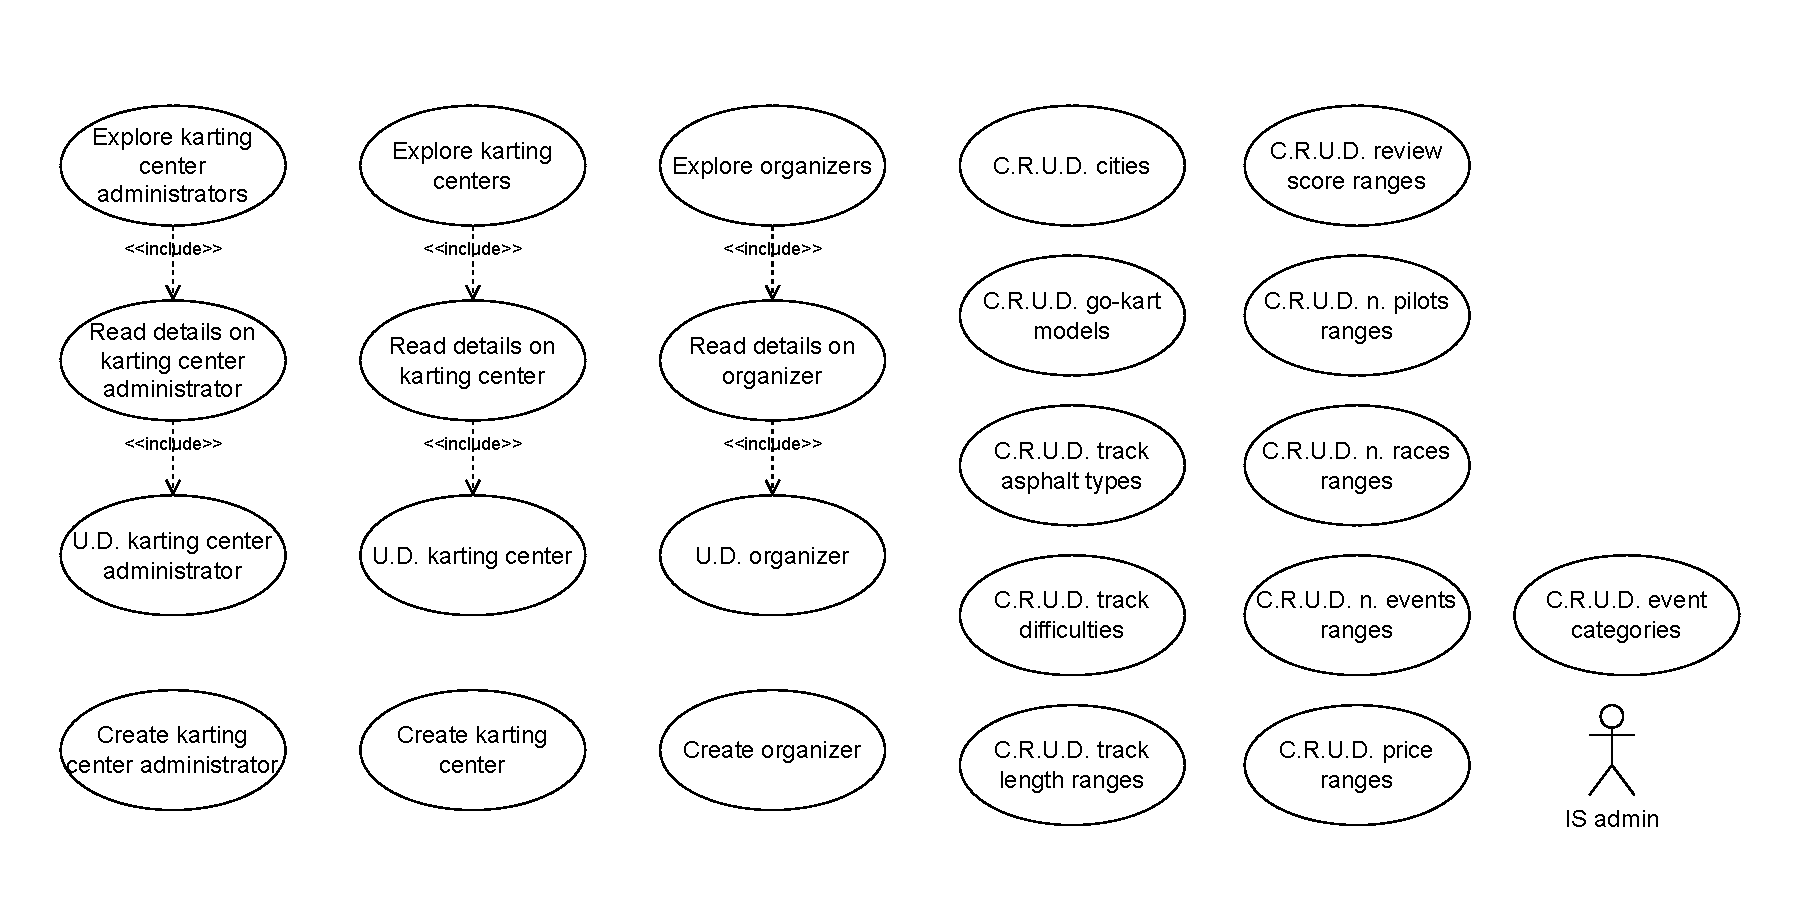
\includegraphics[width=0.7\linewidth]{drawio/is-admin.pdf}
\end{frame}

\subsection*{Extranet}

\begin{frame}
    \frametitle{Organizer}
    \centering
    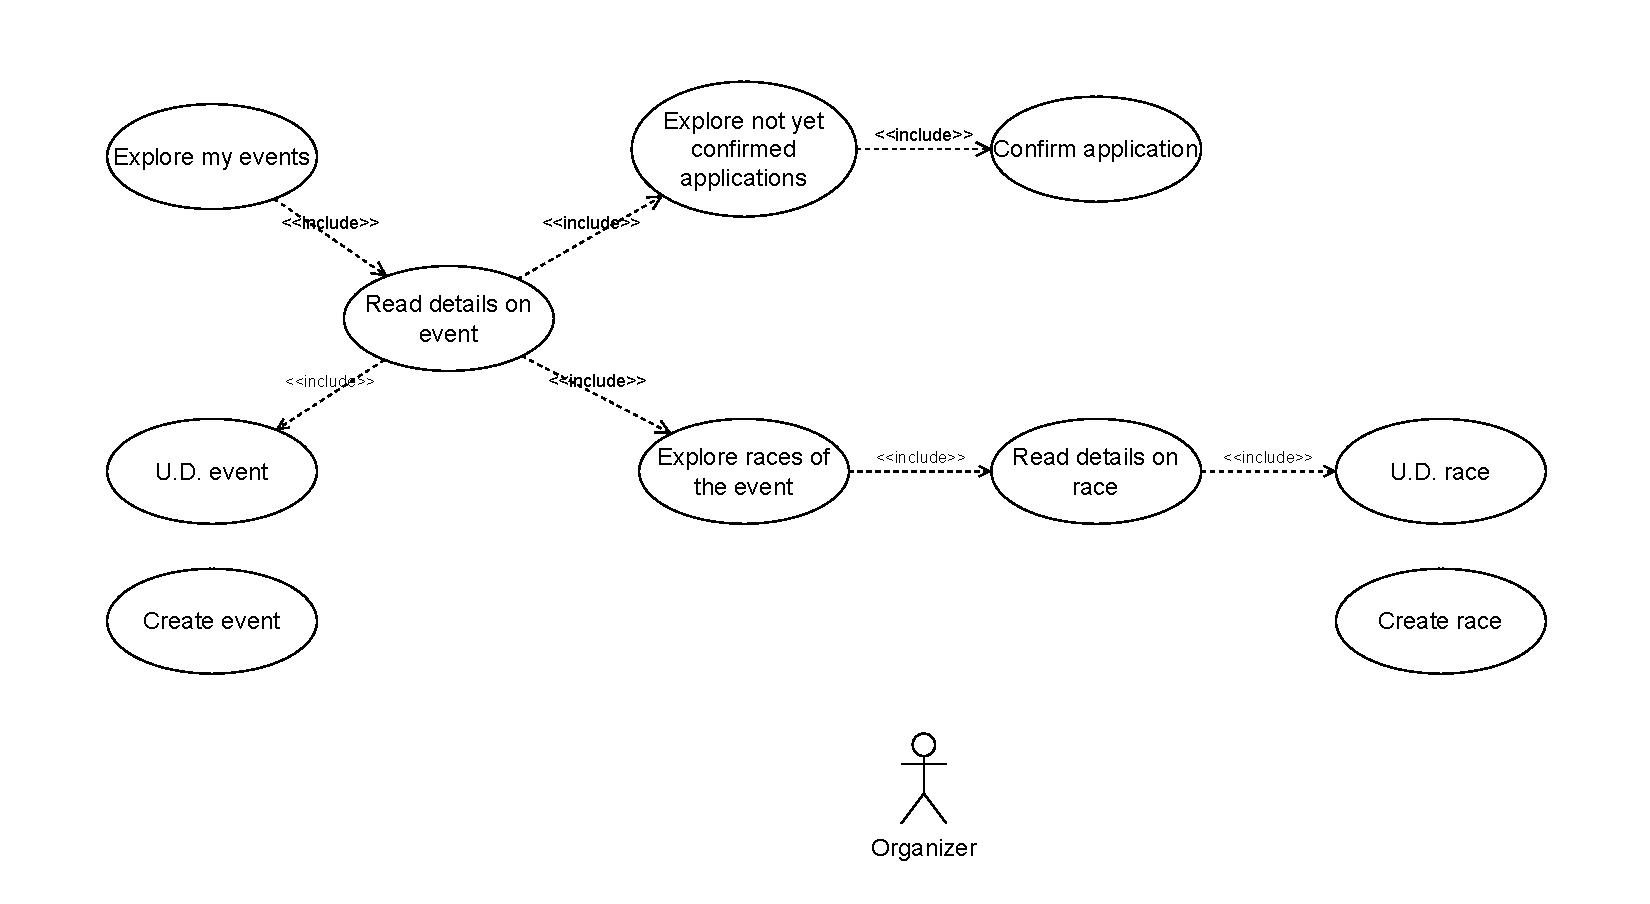
\includegraphics[width=0.9\linewidth]{drawio/organizer.pdf}
\end{frame}


\begin{frame}
    \frametitle{Specification sheet}
    \begin{table}
        \tiny
        \begin{tabular}{|p{2cm}|p{6cm}|}
        \hline
        Title & \textbf{Explore my events} \\
        \hline
        Goal & The user explores the events he created. \\
        \hline
        Precondition & The user logged in and created at least one event.\\
        \hline
        Postcondition & The user obtains the list of events he created. \\
        \hline
        Workflow &
        - A: the user already has a list of events he created and the applications received for each event 
        in the homepage. \newline
        - B: the user moves to the area dedicated to events and the list is already provided. \\
        \hline
        \end{tabular}
\end{table}
\end{frame}


\begin{frame}
    \frametitle{Specification sheet}
    \begin{table}
        \tiny
        \begin{tabular}{|p{2cm}|p{6cm}|}
        \hline
        Title & \textbf{Read details on my event} \\
        \hline
        Goal & The user chooses one event to focus on and reads its details. \\
        \hline
        Precondition & The user logged in. \\
        \hline
        Postcondition & The user obtains the details on the event and 
        can move on to other related informations (e.g. applications). \\
        \hline
        Workflow &
        - A: the user chooses one event from the list of events he created in the homepage. \newline
        - B.1: the user moves to the area dedicated to events. \newline
        - B.2: the user chooses one event from the list of events he created in the area dedicated to events. \\
        \hline
        \end{tabular}
\end{table}
\end{frame}


\begin{frame}
    \frametitle{Specification sheet}
    \begin{table}
        \tiny
        \begin{tabular}{|p{2cm}|p{6cm}|}
        \hline
        Title & \textbf{U.D. events} \\
        \hline
        Goal & The user updates or deletes an event he created. \\
        \hline
        Precondition & The user logged in and he created at least one event. \\
        \hline
        Postcondition & The event is updated or deleted, the modifications might affect the races created for the track 
        and the participations of the pilots to the races of the event but the applications made by pilots are not affected. \\
        \hline
        Workflow &
        - A: the user chooses one event from the list of events he created in the homepage. \newline
        - B.1: the user moves to the area dedicated to events. \newline
        - B.2: the user chooses one event from the list of events he created in the area dedicated to events. \newline
        - The user chooses the option to update or delete the event. \\
        \hline
        \end{tabular}
\end{table}
\end{frame}


\begin{frame}
    \frametitle{Specification sheet}
    \begin{table}
        \tiny
        \begin{tabular}{|p{2cm}|p{6cm}|}
        \hline
        Title & \textbf{Create event} \\
        \hline
        Goal & The user creates a new event. \\
        \hline
        Precondition & The user logged in and created at least one race.\\
        \hline
        Postcondition & The event is created and pilots can apply to it. \\
        \hline
        Workflow &
        - The user moves to the area dedicated to events. \newline
        - The user chooses the option to create a new event (he will need to choose among races he created
        to fill the event). \\
        \hline
        \end{tabular}
\end{table}
\end{frame}

\begin{frame}
    \frametitle{Specification sheet}
    \begin{table}
        \tiny
        \begin{tabular}{|p{2cm}|p{6cm}|}
        \hline
        Title & \textbf{Explore not yet confirmed applications} \\
        \hline
        Goal & The user explores the applications received for his events that he did not confirm yet. \\
        \hline
        Precondition & The user logged in, created at least one event and at least one pilot applied to it.\\
        \hline
        Postcondition & The user obtains the list of applications that he did not confirm yet. \\
        \hline
        Workflow &
        - A: the user chooses one event from the list of events he created in the homepage. \newline
        - B.1: the user moves to the area dedicated to events. \newline
        - B.2: the user chooses one event from the list of events he created in the area dedicated to events. \newline
        (- The list of applications not yet confirmed is already provided.) \\
        \hline
        \end{tabular}
\end{table}
\end{frame}


% \begin{frame}
%     \frametitle{Specification sheet}
%     \begin{table}
%         \tiny
%         \begin{tabular}{|p{2cm}|p{6cm}|}
%         \hline
%         Title & \textbf{Explore not yet confirmed applications} \\
%         \hline
%         Goal & The user explores the applications received for his events that he did not confirm yet. \\
%         \hline
%         Precondition & The user logged in, created at least one event and at least one pilot applied to it.\\
%         \hline
%         Postcondition & The user obtains the list of applications that he did not confirm yet. \\
%         \hline
%         Workflow &
%         - The user follows the same steps as in the use case \textbf{Read details on my event}
%         and the list of applications not yet confirmed is already provided. \\
%         \hline
%         \end{tabular}
% \end{table}
% \end{frame}


\begin{frame}
    \frametitle{Specification sheet}
    \begin{table}
        \tiny
        \begin{tabular}{|p{2cm}|p{6cm}|}
        \hline
        Title & \textbf{Confirm application} \\
        \hline
        Goal & The user confirms an application received for one of his events. \\
        \hline
        Precondition & The user logged in, created at least one event and at least one pilot applied to it.\\
        \hline
        Postcondition & The application is confirmed and the pilot is automatically inserted as a partecipant
        to all of the races of the event (this might change, e.g. in case the organizer decides to organize races 
        in a tournament fashion, but the application will not be affected). \\
        \hline
        Workflow &
        - A: the user chooses one event from the list of events he created in the homepage. \newline
        - B.1: the user moves to the area dedicated to events. \newline
        - B.2: the user chooses one event from the list of events he created in the area dedicated to events. \newline
        - The user chooses the option to accept an application from the list of applications not yet confirmed. \\
        \hline
        \end{tabular}
\end{table}
\end{frame}

\begin{frame}
    \frametitle{Specification sheet}
    \begin{table}
        \tiny
        \begin{tabular}{|p{2cm}|p{6cm}|}
        \hline
        Title & \textbf{Explore races of the event} \\
        \hline
        Precondition & The user logged in, created at least one event and the event has at least one race. \\
        \hline
        Postcondition & The user obtains the list of races of a specific event. \\
        \hline
        Workflow &
        - A: the user chooses one event from the list of events he created in the homepage. \newline
        - B.1: the user moves to the area dedicated to events. \newline
        - B.2: the user chooses one event from the list of events he created in the area dedicated to events. \newline
        (- The list of races of the chosen event is already provided.) \\
        \hline
        \end{tabular}
\end{table}
\end{frame}

\begin{frame}
    \frametitle{Specification sheet}
    \begin{table}
        \tiny
        \begin{tabular}{|p{2cm}|p{6cm}|}
        \hline
        Title & \textbf{Read details on race} \\
        \hline
        Precondition & The user logged in, created at least one event and the event has at least one race. \\
        \hline
        Postcondition & The user obtains the details on the race and can move on (e.g. updating or deleting it.) \\
        \hline
        Workflow &
        - A: the user chooses one event from the list of events he created in the homepage. \newline
        - B.1: the user moves to the area dedicated to events. \newline
        - B.2: the user chooses one event from the list of events he created in the area dedicated to events. \newline
        - The user chooses one race from the list of races of the chosen event. \\
        \hline
        \end{tabular}
\end{table}
\end{frame}


\begin{frame}
    \frametitle{Specification sheet}
    \begin{table}
        \tiny
        \begin{tabular}{|p{2cm}|p{6cm}|}
        \hline
        Title & \textbf{U.D. race} \\
        \hline
        Precondition & The user logged in, created at least one event and the event has at least one race. \\
        \hline
        Postcondition & The race gets updated or deleted, this affects the relations with the pilots (\textit{partecipation})
        but not the application of the pilots to the event. \\
        \hline
        Workflow &
        - A: the user chooses one event from the list of events he created in the homepage. \newline
        - B.1: the user moves to the area dedicated to events. \newline
        - B.2: the user chooses one event from the list of events he created in the area dedicated to events. \newline
        - The user chooses one race from the list of races of the chosen event. \newline
        - The user chooses the option to update or delete the race. \\
        \hline
        \end{tabular}
\end{table}
\end{frame}

\begin{frame}
    \frametitle{Specification sheet}
    \begin{table}
        \tiny
        \begin{tabular}{|p{2cm}|p{6cm}|}
        \hline
        Title & \textbf{Create race} \\
        \hline
        Precondition & The user logged in. \\
        \hline
        Postcondition & A new race is available to the user to be added to an event. \\
        \hline
        Workflow &
        - The user moves to the area dedicated to events. \newline
        - The user chooses the option to create a new race. \\
        \hline
        \end{tabular}
\end{table}
\end{frame}


\subsection*{Internet}

\begin{frame}
    \frametitle{Pilot}
    \centering
    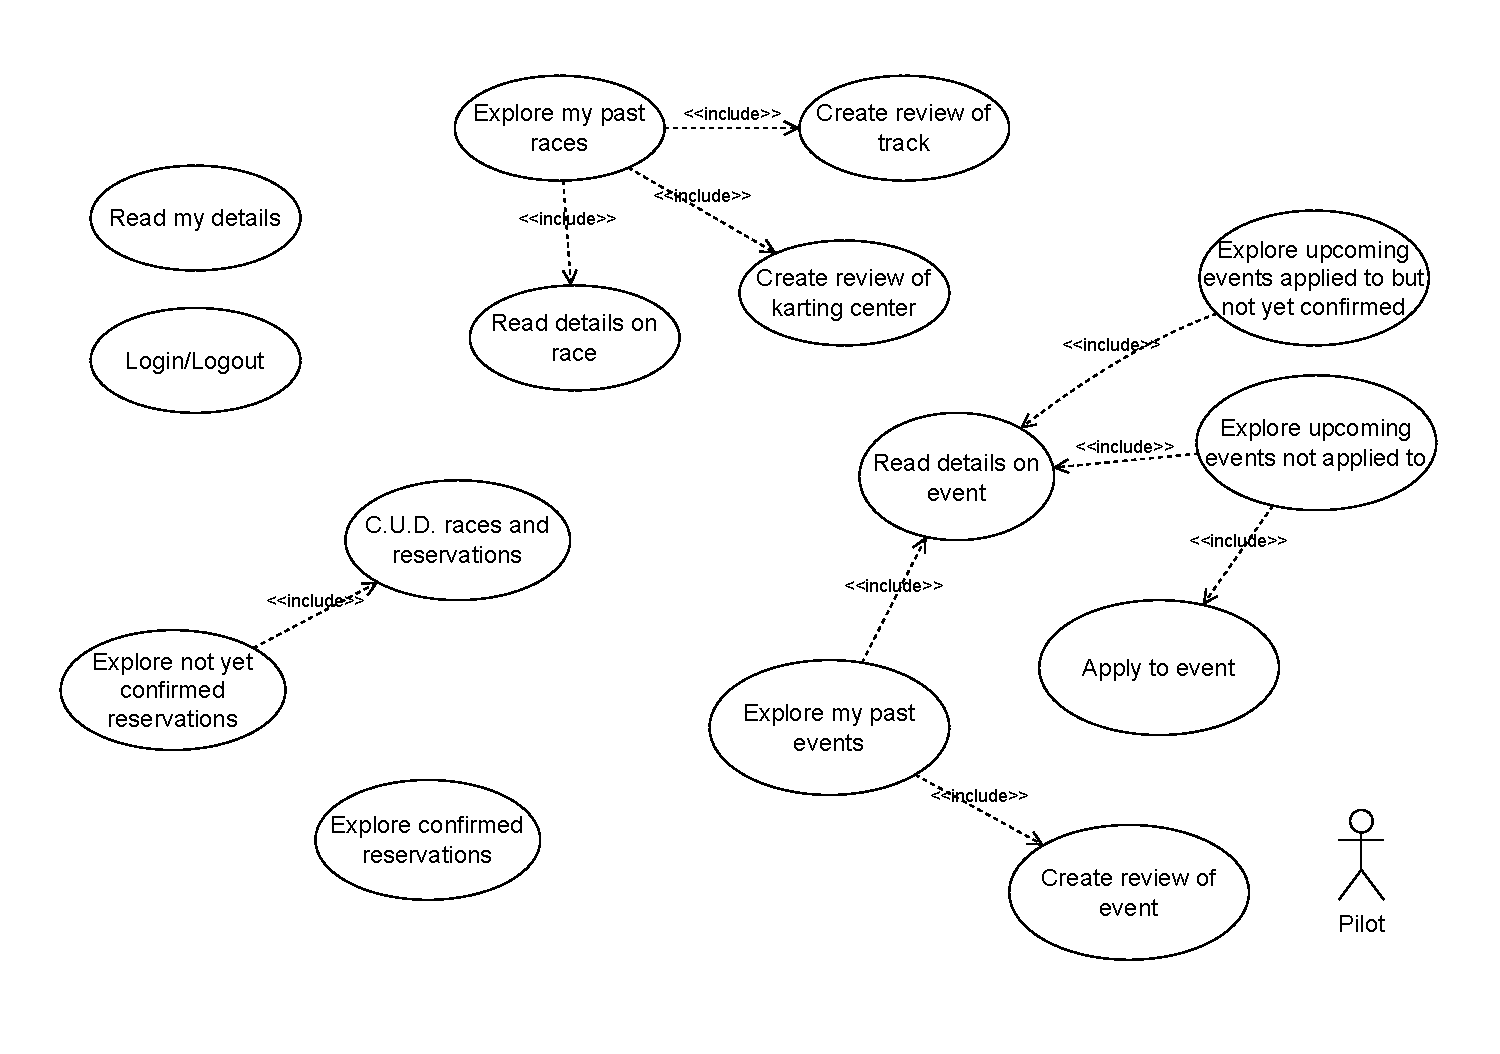
\includegraphics[width=0.9\linewidth]{drawio/pilot.pdf}
\end{frame}

% %%%%% PILOT USE CASE SHEET %%%%%

\begin{frame}
    \frametitle{Specification sheet}
    \begin{table}
        \tiny
        \begin{tabular}{|p{2cm}|p{6cm}|}
        \hline
        Title & \textbf{Read my details} \\
        \hline
        Goal & The user reads its own personal informations, already available in the homepage.\\
        \hline
        Precondition & The user logged in. \\
        \hline
        Postcondition & The user obtains its personal informations. \\
        \hline
        Workflow &
        - The user logs in and reads the informations already present in the homepage. \\
        \hline
        \end{tabular}
\end{table}
\end{frame}

\begin{frame}
    \frametitle{Specification sheet}
    \begin{table}
        \tiny
        \begin{tabular}{|p{2cm}|p{6cm}|}
        \hline
        Title & \textbf{Explore not yet confirmed reservations} \\
        \hline
        Goal & The user explores the reservations he made that are not yet confirmed by any clerk \\
        \hline
        Precondition & The user logged in. \\
        \hline
        Postcondition & The user obtains the list of reservations that are not yet confirmed by any clerk. \\
        \hline
        Workflow &
        - The user moves to the area dedicated to reservations and the list is already provided. \\
        \hline
        \end{tabular}
\end{table}
\end{frame}


\begin{frame}
    \frametitle{Specification sheet}
    \begin{table}
        \tiny
        \begin{tabular}{|p{2cm}|p{6cm}|}
        \hline
        Title & \textbf{C.U.D. races and reservations} \\
        \hline
        Goal & The user asks for a reservation to have a race on a track of a karting center. \\
        \hline
        Precondition & The user logged in. \\
        \hline
        Postcondition & A race and its relative reservation (a weak entity of the race) are created, updated or deleted. \\
        \hline
        Workflow &
        - The user moves to the area dedicated to reservations. \newline
        - A: the user selects a reservation from those not yet confirmed and updates it or deletes it. \newline
        - B: the user creates a new reservation without the need to select one from those not yet confirmed. \newline
        Note: the existence of the reservation is hidden to the user when he creates/updates/deletes the race,
        the reservation just takes some of the attributes of the race (Date, Start, End) and is shared with the clerks
        of the karting center, who can confirm it or not. The user can only see the reservations that are
        confirmed or not, he does not edit them directly but only through the actions on the race. \\
        \hline
        \end{tabular}
\end{table}
\end{frame}


\begin{frame}
    \frametitle{Specification sheet}
    \begin{table}
        \tiny
        \begin{tabular}{|p{2cm}|p{6cm}|}
        \hline
        Title & \textbf{Explore confirmed reservations} \\
        \hline
        Goal & The user explores the reservations he made that are confirmed by a clerk \\
        \hline
        Precondition & The user logged in. \\
        \hline
        Postcondition & The user obtains the list of reservations that are confirmed by a clerk. \\
        \hline
        Workflow &
        - The user moves to the area dedicated to reservations and the list is already provided. \\
        \hline
        \end{tabular}
\end{table}
\end{frame}

\begin{frame}
    \frametitle{Specification sheet}
    \begin{table}
        \tiny
        \begin{tabular}{|p{2cm}|p{6cm}|}
        \hline
        Title & \textbf{Explore my past races} \\
        \hline
        Goal & The user explores the races he had in the past (not the races he booked through the previous 
        use case). \\
        \hline
        Precondition & The user logged in. \\
        \hline  
        Postcondition & The user obtains the list of past races. \\
        \hline
        Workflow &
        - The user moves to the area dedicated to races
        and the list is already provided. \\
        \hline
        \end{tabular}
\end{table}
\end{frame}

\begin{frame}
    \frametitle{Specification sheet}
    \begin{table}
        \tiny
        \begin{tabular}{|p{2cm}|p{6cm}|}
        \hline
        Title & \textbf{Read details on race} \\
        \hline
        Goal & The user chooses one race to focus on and reads its details. \\
        \hline
        Precondition & The user logged in. \\
        \hline
        Postcondition & The user obtains the details on the race and related informations such as the best lap-time of
        that race (it could be from the user himself or another pilot). \\
        \hline
        Workflow &
        - The user moves to the area dedicated to races. \newline
        - The user chooses one race from the list of past races. \\
        \hline
        \end{tabular}
\end{table}
\end{frame}


\begin{frame}
    \frametitle{Specification sheet}
    \begin{table}
        \tiny
        \begin{tabular}{|p{2cm}|p{6cm}|}
        \hline
        Title & \textbf{Create review of karting center} \\
        \hline
        Goal & The user creates a review of a karting center. \\
        \hline
        Precondition & The user logged in and had at least one race that will allow him to write 
        reviews for the track and the karting center that hosted that race. \\
        \hline
        Postcondition & The review is stored and a clerk of the karting center will be able to 
        read it and remove it if it is considered inappropriate. \\
        \hline
        Workflow &
        - The user moves to the area dedicated to reviews. \newline
        - From the list of past races, the user selects the option to write a review of the karting center that
        hosted the chosen race from the list. \newline
        - The user chooses a score, writes the review and submits it. \\
        \hline
        \end{tabular}
    \end{table}

    \begin{table}
        \tiny
        \begin{tabular}{|p{2cm}|p{6cm}|}
        \hline
        Title & \textbf{Create review of track} \\
        \hline
        Goal, precondition, postcondition, workflow & Equivalent to the previous use case, but the review is of a track. \\
        \hline
        \end{tabular}
    \end{table}
\end{frame}

\begin{frame}
    \frametitle{Specification sheet}
    \begin{table}
        \tiny
        \begin{tabular}{|p{2cm}|p{6cm}|}
        \hline
        Title & \textbf{Explore upcoming events applied to but not confirmed yet} \\
        \hline
        Goal & The user explores the events that he applied to 
        and that have not been confirmed by an organizer yet. \\
        \hline
        Precondition & The user logged in. \\
        \hline
        Postcondition & The user obtains the list of events that he 
        applied to and that have not been confirmed yet. \\
        \hline
        Workflow &
        - The user moves to the area dedicated to events and the list is already provided. \\
        \hline
        \end{tabular}
    \end{table}
\end{frame}


\begin{frame}
    \frametitle{Specification sheet}
    \begin{table}
        \tiny
        \begin{tabular}{|p{2cm}|p{6cm}|}
        \hline
        Title & \textbf{Explore upcoming events not applied to} \\
        \hline
        Goal & The user explores the upcoming events that he did not apply to. \\
        \hline
        Precondition & The user logged in. \\
        \hline
        Postcondition & The user obtains the list of upcoming events that he did not apply to. \\
        \hline
        Workflow &
        - The user moves to the area dedicated to events and the list is already provided. \\
        \hline
        \end{tabular}
    \end{table}
\end{frame}


\begin{frame}
    \frametitle{Specification sheet}
    \begin{table}
        \tiny
        \begin{tabular}{|p{2cm}|p{6cm}|}
        \hline
        Title & \textbf{Explore my past events} \\
        \hline
        Goal & The user explores the events that he attended in the past. \\
        \hline
        Precondition & The user logged in and attended at least one event in the past. \\
        \hline
        Postcondition & The user obtains the list of events that he attended in the past. \\
        \hline
        Workflow &
        - The user moves to the area dedicated to events. \newline
        - The user selects the option to explore the events that he attended in the past. \\
        \hline
        \end{tabular}
    \end{table}
\end{frame}


\begin{frame}
    \frametitle{Specification sheet}
    \begin{table}
        \tiny
        \begin{tabular}{|p{2cm}|p{6cm}|}
        \hline
        Title & \textbf{Apply to an event} \\
        \hline
        Goal & The user applies to an event. \\
        \hline
        Precondition & The user logged in and he has not already applied to the event. \\
        \hline
        Postcondition & The user applies to the event and the organizer will be able to see and confirm the application. \\
        \hline
        Workflow &
        - The user moves to the area dedicated to events. \newline
        - The user selects one event from the list of upcoming events that he did not apply to. \newline
        - The user applies to the event. \\
        \hline
        \end{tabular}
    \end{table}
\end{frame}

\begin{frame}
    \frametitle{Specification sheet}
    \begin{table}
        \tiny
        \begin{tabular}{|p{2cm}|p{6cm}|}
        \hline
        Title & \textbf{Read details on event} \\
        \hline
        Goal & The user chooses one event to focus on and reads its details. \\
        \hline
        Precondition & The user logged in. \\
        \hline
        Postcondition & The user obtains the details on the event. \\
        \hline
        Workflow &
        - The user moves to the area dedicated to events. \newline
        - A: the user chooses one event from the list of upcoming events (both applied to and not applied to). \newline
        - B.1: the user chooses the option to explore the events that he attended in the past. \newline
        - B.2: the user chooses one event from the list of past events. \\
        \hline
        \end{tabular}
    \end{table}
\end{frame}

\begin{frame}
    \frametitle{Specification sheet}
    \begin{table}
        \tiny
        \begin{tabular}{|p{2cm}|p{6cm}|}
        \hline
        Title & \textbf{Create review of event} \\
        \hline
        Goal & The user creates a review of an event he has attended in the past. \\
        \hline
        Precondition & The user logged in and attended at least one event in the past. \\
        \hline
        Postcondition & The review is stored and the organizer of the event and the clerks of all the 
        karting centers that hosted at least one race of the event will be able to read it, clerks will 
        be able to remove it if it is considered inappropriate. \\
        \hline
        Workflow &
        - The user moves to the area dedicated to events. \newline
        - The user chooses the option to explore the events that he attended in the past. \newline
        - The user selects the option to write a review from one of the events in the list. \newline
        - The user chooses a score, writes the review and submits it. \\
        \hline
        \end{tabular}
    \end{table}
\end{frame}



\begin{frame}
    \frametitle{Visitor}
    \centering
    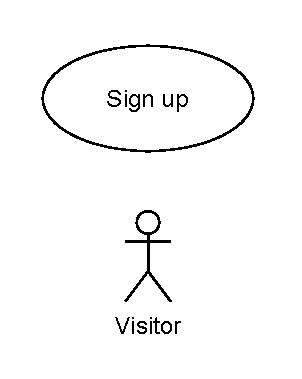
\includegraphics[width=0.3\linewidth]{drawio/visitor.pdf}
\end{frame}

\begin{frame}
\frametitle{Karting center administrator}

\begin{table}
    \tiny
    \begin{tabular}{|p{2cm}|p{6cm}|}
    \hline
    Group name & \textbf{Karting center administrator} \\
    \hline
    Profile data & Name, Surname, e-mail address, password, address, phone number \\
    \hline
    Super group & Intranet \\
    \hline
    Sub group & None \\
    \hline
    Relevant use cases & CRUD on events, races, pilots, tracks, leaderboard, 
    login, logout \\
    \hline
    Read & All \\
    \hline
    Write & All \\
    \hline
    \end{tabular}
    \end{table}
\end{frame}

\begin{frame}
\frametitle{Pilot}

\begin{table}
    \tiny
    \begin{tabular}{|p{2cm}|p{6cm}|}
    \hline
    Group name & \textbf{Pilot} \\
    \hline
    Profile data & Name, Surname, e-mail address, password, address, phone number \\
    \hline
    Super group & Internet \\
    \hline
    Sub group & None \\
    \hline
    Relevant use cases & Create a race, Apply for an event, 
    login, logout \\
    \hline
    Read & All \\
    \hline
    Write & Race, Leaderboard \\
    \hline
    \end{tabular}
    \end{table}

\end{frame}




\section*{Data dictionary}
\begin{frame}
\frametitle{Karting center}

% Table with two columns and 9 rows:
% - Name
% - Synonym
% - Description
% - Example of instance
% - Properties
% - Components
% - Relations
% - Superconcepts
% - Subconcepts

% table 9x2
\begin{table}
\tiny
\begin{tabular}{|p{2cm}|p{6cm}|}
\hline
Name & \textbf{Karting center} \\
\hline
Synonym & Go-karting center \\
\hline
Description & Karting center \\
\hline
Example of instance & 
Name: Mantova Karting Center \newline
\textit{City}: Mantova \newline
\textit{nPilots}: 5937 \newline
\textit{nRaces}: 12485 \newline
\textit{nEvents}:74 \newline
\textit{avgReviewScore}: 3.9 \\
\hline
Properties & 
Name: the name of the karting center\newline
\textit{City}: the city where the karting center is located\newline
\textit{nPilots}: the number of pilots that have raced in the karting center \newline
\textit{nRaces}: the number of races that took place in the karting center \newline
\textit{nEvents}: the number of events that had at least one race hosted by the karting center \newline
\textit{avgReviewScore}: the average score of the reviews of the karting center \\
\hline
Components & None \\
\hline
\end{tabular}
\end{table}

\end{frame}

\begin{frame}
\begin{table}
\tiny
\begin{tabular}{|p{2cm}|p{6cm}|}
\hline
Relations &
KartingCenter\_City (N:1): the city where the karting center is located \newline
KartingCenter\_KartingCenterAdmin (N:1): the karting center administrator of the karting center \newline
KartingCenter\_Clerk (1:N): the clerks of the karting center \newline
KartingCenter\_KartingCenterReview (1:N): the reviews of the karting center \newline
KartingCenter\_Track (1:N): the tracks of the karting center \newline
\textit{KartingCenter\_NPilotsRange} (N:1) the range within the number of pilots that have raced in the karting center falls \newline
\textit{KartingCenter\_NRacesRange} (N:1) the range within the number of races that took place in the karting center falls \newline
\textit{KartingCenter\_NEventsRange} (N:1) the range within the number of events that took place in the karting center falls \newline
\textit{KartingCenter\_KCReviewScoreRange} (N:1) the range within the average score of the reviews of the karting center falls \newline
\textit{KartingCenter\_Event} (N:N) the events the karting center hosted \\
\hline
Superconcepts & None \\
\hline
Subconcepts & None \\
\hline
\end{tabular}
\end{table}
\end{frame}

\begin{frame}
\frametitle{City}
\begin{table}
\tiny
\begin{tabular}{|p{2cm}|p{6cm}|}
\hline
Name & \textbf{City} \\
\hline
Synonym & None \\
\hline
Description & City \\
\hline
Example of instance & 
Name: Mantova \\
\hline
Properties & 
Name: the name of the city \\
\hline
Components & None \\
\hline
Relations &
City\_KartingCenter (1:N): the karting centers located in the city \newline
\textit{City\_Track} (1:N): the tracks (inside a karting center) located in the city \newline
\textit{City\_Event} (N:N): the events that had at least one race on a track of a karting center
located in the city \\
\hline
Superconcepts & None \\
\hline
Subconcepts & None \\
\hline
\end{tabular}
\end{table}
\end{frame}

\begin{frame}
\frametitle{Track}
\begin{table}
\tiny
\begin{tabular}{|p{2cm}|p{6cm}|}
\hline
Name & \textbf{Track} \\
\hline
Synonym & Circuit \\
\hline
Description & Track \\
\hline
Example of instance &
Name: T1 \newline
Length: 700m \newline
\textit{City}: Mantova \newline
\textit{AsphaltType}: resin \newline
\textit{nRentalGoKarts}: 23 \newline
\textit{Difficulty}: Intermediate \newline
\textit{nPilots}: 3873 \newline
\textit{nRaces}: 7437 \newline
\textit{nEvents}: 43 \newline
\textit{avgReviewScore}: 4.2 \\
\hline
Properties &
Name: the name of the track \newline
Length: the length of the track \newline
\textit{City}: the city where the karting center the track belongs to is located \newline
\textit{AsphaltType}: the type of asphalt of the track \newline
\textit{nRentalGoKarts}: the number of rental go-karts available in the track \newline
\textit{Difficulty}: the difficulty of the track \newline
\textit{nPilots}: the number of pilots that have raced on the track \newline
\textit{nRaces}: the number of races that took place on the track \newline
\textit{nEvents}: the number of events that had at least one race on the track \newline
\textit{avgReviewScore}: the average score of the reviews of the track \\
\hline
Components & 
Timetable: the timetable of the track \newline
Leaderboard: a leaderboard of the track \\
\hline
\end{tabular}
\end{table}
\end{frame}

\begin{frame}
\begin{table}
\tiny
\begin{tabular}{|p{2cm}|p{6cm}|}
\hline
Relations &
Track\_KartingCenter (N:1): the karting center the track belongs to \newline
Track\_TrackReview (1:N): the reviews of the track \newline
Track\_Timetable (1:1): the timetable of the track \newline
Track\_Leaderboard (1:N): the leaderboards of the track \newline
Track\_Race (1:N): the races that took place on the track \newline
Track\_GoKart (1:N): the go-karts dedicated to the track \newline
Track\_GoKartModel (N:N): the go-kart models allowed on the track \newline
Track\_TrackAshpalt (N:1): the asphalt of the track \newline
Track\_TrackDifficulty (N:1): the difficulty of the track \newline
Track\_Pilot (N:N): the pilots that have the track as one of their favorite \newline
\textit{Track\_City} (N:1): the city where the karting center the track belongs to is located \newline
\textit{Track\_TrackLengthRange} (N:1): the range within the length of the track falls \newline
\textit{Track\_NPilotsRange} (N:1): the range within the number of pilots that have raced on the track falls \newline
\textit{Track\_NRacesRange} (N:1): the range within the number of races that took place on the track falls \newline
\textit{Track\_NEventsRange} (N:1): the range within the number of events that took place on the track falls \newline
\textit{Track\_TrackReviewScoreRange} (N:1): the range within the average score of the reviews of the track falls \\
\hline
Superconcepts & None \\
\hline
Subconcepts & 
Popular track: a track that is recurrent in the list of favorite tracks of pilots \\
\hline
\end{tabular}
\end{table}
\end{frame}

\begin{frame}
\frametitle{Go-kart}
\begin{table}
\tiny
\begin{tabular}{|p{2cm}|p{6cm}|}
\hline
Name & \textbf{Go-kart} \\
\hline
Synonym & Kart \\
\hline
Description & Go-kart \\
\hline
Example of instance &
Name: T1.1 \newline
GoKartModel: Sodi RX7 \\
\hline
Properties &
Name: the name of the go-kart \newline
\textit{GoKartModel}: the model of the go-kart \\
\hline
Components & None \\
\hline
Relations &
GoKart\_Track (N:1): the track the go-kart is dedicated to \newline
GoKart\_GoKartModel (N:1): the model of the go-kart \\
\hline
Superconcepts & None \\
\hline
Subconcepts & None \\
\hline
\end{tabular}
\end{table}
\end{frame}

\begin{frame}
\frametitle{Timetable}
\begin{table}
\tiny
\begin{tabular}{|p{2cm}|p{6cm}|}
\hline
Name & \textbf{Timetable} \\
\hline
Synonym & None \\
\hline
Description & Timetable \\
\hline
Example of instance &
\textit{TrackName}: T1 \\
\hline
Properties &
\textit{TrackName}: the name of the track \\
\hline
Components & None \\
\hline
Relations &
Timetable\_Track (1:1): the track the timetable belongs to \newline
Timetable\_Reservation (1:N): the reservations of the timetable \\
\hline
Superconcepts & None \\
\hline
Subconcepts & None \\
\hline
\end{tabular}
\end{table}
\end{frame}

\begin{frame}
\frametitle{Leaderboard}
\begin{table}
\tiny
\begin{tabular}{|p{2cm}|p{6cm}|}
\hline
Name & \textbf{Leaderboard} \\
\hline
Synonym & Ranking \\
\hline
Description & Leaderboard \\
\hline
Example of instance &
Title: Best of the week \newline
\textit{TrackName}: T1 \\
\hline
Properties &
Title: the title of the leaderboard \newline
\textit{TrackName}: the name of the track \\
\hline
Components & None \\
\hline
Relations &
Leaderboard\_Track (N:1): the track each leaderboard belongs to \newline
\textit{Leaderboard\_LapTime} (1:N): the lap times the leaderboard focuses on \\
\hline
Superconcepts & None \\
\hline
Subconcepts & None \\
\hline
\end{tabular}
\end{table}
\end{frame}

\begin{frame}
\frametitle{Race}
\begin{table}
\tiny
\begin{tabular}{|p{2cm}|p{6cm}|}
\hline
Name & \textbf{Race} \\
\hline
Synonym & None \\
\hline
Description & Race \\
\hline
Example of instance &
ID: 2036 \newline
Date: 2024-02-15 \newline
Start: 15:00 \newline
End: 15:09 \newline
ForEvent: false \newline
\textit{GoKartingCenterName}: Mantova Karting Center \newline
\textit{TrackName}: T1 \newline
\textit{nPartecipants}: 8 \newline
\textit{fastestLapTime}: 00:00:48.595 \\
\hline
Properties &
ID \newline
Date \newline
Start \newline
End \newline
ForEvent: whether the race was created by an organizer for an event or not \newline
\textit{GoKartingCenterName} \newline
\textit{TrackName}: the name of the track that hosts the race \newline
\textit{nPartecipants} \newline
\textit{fastestLapTime} \\
\hline
Components & None \\
\hline
\end{tabular}
\end{table}
\end{frame}

\begin{frame}
\begin{table}
\tiny
\begin{tabular}{|p{2cm}|p{6cm}|}
\hline
Relations & 
Race\_Track (N:1): the track the race has been raced on \newline
Race\_Reservation (1:1): the reservation that has been made for the race \newline
Race\_Pilot (1:N): the pilots that participated in the race \newline
Race\_Pilot (N:1): the pilot who has this race as his/her last race \newline
Race\_LapTime (1:N): every lap-time of every pilot that participated in the race \newline
Race\_Event (N:1): the event the race is part of \\
\hline
Superconcepts & None \\
\hline
Subconcepts & None \\
\hline
\end{tabular}
\end{table}
\end{frame}

\begin{frame}
\frametitle{Reservation}
\begin{table}
\tiny
\begin{tabular}{|p{2cm}|p{6cm}|}
\hline
Name & \textbf{Reservation} \\
\hline
Synonym & Booking \\
\hline
Description & Reservation \\
\hline
Example of instance &
Date: 2024-02-15 \newline
Start: 15:00 \newline
End: 15:09 \newline
\textit{ReservedByPilot}: Denis Festa \newline
\textit{ReservedByOrganizer}: None \newline
\textit{ConfirmedByClerk}: Jessica \\
\hline
Properties &
Date \newline
Start \newline
End \newline
\textit{ReservedByPilot}: the pilot who made the reservation (this property 
is mutually exclusive with \textit{ReservedByOrganizer}) \newline
\textit{ReservedByOrganizer}: the organizer who made the reservation (this property
is mutually exclusive with \textit{ReservedByPilot}) \newline
\textit{ConfirmedByClerk}: the clerk who confirmed the reservation \\
\hline
Components & None \\
\hline
Relations &
Reservation\_Timetable (N:1): the timetable where the reservation is stored \newline
Reservation\_Pilot (N:1): the pilot who made the reservation \newline
Reservation\_Organizer (N:1): the organizer who made the reservation \newline
Reservation\_Clerk (N:1): the clerk who confirmed the reservation \newline
Reservation\_Race (N:1): the race this reservation has been made for \\
\hline
Superconcepts & None \\
\hline
Subconcepts & None \\
\hline
\end{tabular}
\end{table}
\end{frame}

\begin{frame}
\frametitle{Lap-time}
\begin{table}
\tiny
\begin{tabular}{|p{2cm}|p{6cm}|}
\hline
Name & \textbf{Lap-time} \\
\hline
Synonym & Lap \\
\hline
Description & Lap-time \\
\hline
Example of instance &
LapNumber: 7 \newline
LapTime: 00:00:48.595 \\
\hline
Properties &
LapNumber: the \textit{LapNumber}-th lap \newline
LapTime: the time measured for the \textit{LapNumber}-th lap for 
a particular pilot \\
\hline
Components & None \\
\hline
Relations & 
LapTime\_Pilot (N:1): the pilot who made the lap-time \newline
LapTime\_Race (N:1): the race where the lap-time has been made \newline
\textit{LapTime\_Leaderboard} (N:N): the leaderboards where the lap-time is displayed \\
\hline
Superconcepts & None \\
\hline
Subconcepts & None \\
\hline
\end{tabular}
\end{table}
\end{frame}

\begin{frame}
\frametitle{Application}
\begin{table}
\tiny
\begin{tabular}{|p{2cm}|p{6cm}|}
\hline
Name & \textbf{Application} \\
\hline
Synonym & Request \\
\hline
Description & Application \\
\hline
Example of instance &
Confirmed: true \newline
\textit{EventName}: Mantova Karting Cup 2024 \newline
\textit{RequestFromPilot}: Denis Festa \\
\hline
Properties &
Confirmed: whether the application has been confirmed or not (the organizer who
created the event is the
only one who can accept an application) \newline
\textit{EventName}: the name of the event the application has been made for \newline
\textit{RequestFromPilot}: the pilot who made the application \\
\hline
Components & None \\
\hline
Relations &
Application\_Pilot (N:1): the pilot who made the application \newline
Application\_Event (N:1): the event the application has been made for \\
\hline
Superconcepts & None \\
\hline
Subconcepts & None \\
\hline
\end{tabular}
\end{table}
\end{frame}

\begin{frame}
\frametitle{Event}
\begin{table}
\tiny
\begin{tabular}{|p{2cm}|p{6cm}|}
\hline
Name & Event \\
\hline
Synonym & Tournament \\
\hline
Description & Event \\
\hline
Example of instance &
Name: Mantova Karting Cup 2024 \newline
Price: 100 \newline
\textit{FirstDate}: 2024-02-15 \newline
\textit{OrganizerName}: WD40 \newline
\textit{EventCategory}: Open \newline
\textit{nPartecipants}: 64 \newline
\textit{nRaces}: 12 \newline
\textit{nReviews}: 23 \newline
\textit{avgReviewScore}: 4.5 \\
\hline
Properties &
Name: the name of the event \newline
Price: the price of the event \newline
\textit{FirstDate}: the date of the first race of the event \newline
\textit{OrganizerName}: the username of the organizer who created the event \newline
\textit{EventCategory}: the category of the event (\textit{open, intermediate, pro})\newline
\textit{nPartecipants}: the number of pilots who applied for the event and whose application was confirmed\newline
\textit{nRaces}: the number of races of the event \newline
\textit{nReviews}: the number of written reviews about the event \newline
\textit{avgReviewScore}: the average score of the reviews about the event \\
\hline
Components & None \\
\hline
\end{tabular}
\end{table}
\end{frame}

\begin{frame}
\begin{table}
\tiny
\begin{tabular}{|p{2cm}|p{6cm}|}
\hline
Relations &
Event\_Organizer (N:1): the organizer who created the event \newline
Event\_Application (1:N): the applications received for the event \newline
Event\_Race (1:N): the races of the event \newline
Event\_EventCategory (N:1): the category of the event \newline
Event\_EventReview (1:N): the reviews about the event \newline
\textit{Event\_EReviewScoreRange} (N:1): the range within the average score of the reviews about the event falls \newline
\textit{Event\_Pilot} (N:N): the pilots who applied for the event and whose application was confirmed \newline
\textit{Event\_PriceRange} (N:1): the range within the price of the event falls \newline
\textit{Event\_City} (N:N): the cities where the races of the event took place \newline
\textit{Event\_Track} (N:N): the tracks that hosted the races of the event \newline
\textit{Event\_KartingCenter} (N:N): the karting centers whose tracks hosted the races of the event \\
\hline
Superconcepts & None \\
\hline
Subconcepts & Controversial event, Popular evenet, Upcoming event \\
\hline
\end{tabular}
\end{table}
\end{frame}










% Quando voglio visitare un nuovo arrivo
% utilizzo non una query ma una derivata
% che calcola la query una volta sola

\end{document}